\section{汽油机的工作原理}\label{sec:6-1}

内燃机的基本特点是让燃料在机器的气缸内燃烧,生成高温高压的燃气,
利用这个燃气作为工作物质去推动活塞做功。内燃机的名字就是由此而来的。

\begin{wrapfigure}{r}{6.5cm}
    \centering
    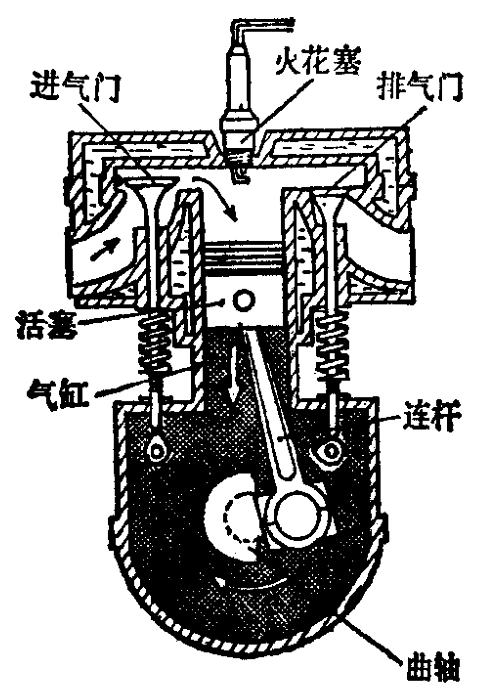
\includegraphics[width=5cm]{../pic/czwl2-ch6-1}
    \caption{}\label{fig:6-1}
\end{wrapfigure}

内燃机有两种:汽油机和柴油机。这一节,我们介绍汽油机的工作原理。

汽油机是用汽油作燃料的内燃机。它的构造如图 \ref{fig:6-1} 所示,气缸里的活塞用连杆跟曲轴相连,
气缸上面有进气门和排气门,气缸顶部有火花塞。

汽油机工作的时候,活塞在气缸里往复运动。活塞从气缸一端运动到另一端叫做一个冲程。
四冲程汽油机的工作过程是由吸气、压缩、做功、排气四个冲程组成的。

第一个冲程是吸气冲程。如 \hyperref[fig:pic3]{彩图3} 甲所示,
进气门打开,排气门关闭,活塞由最上端向下运动,气缸里气体的体积增大,压强减小(低于大气压),
于是在化油器内由汽油和空气形成的燃料混合物从进气门被吸入气缸。
当活塞到达气缸最下端的时候,进气门关闭,完成吸气冲程。

第二个冲程是压缩冲程。 如 \hyperref[fig:pic3]{彩图3} 乙所示,
进气门和排气门都关闭,活塞向上运动,燃料混合物受到压缩,压强和温度都提高了。
最后压强达到 6~15千克力/$\pflm$\footnotemark,温度升高到 250 ~ 300 ℃ 左右。
\footnotetext{千克力/$\pflm$ (即工程大气压)是工程技术上常用的压强单位,
它与帕斯卡的关系是: $1 \text{千克力/}\pflm = 9.80665 \times 10^4 \pasika$。}

第三个冲程是做功冲程。如 \hyperref[fig:pic3]{彩图3} 丙所示,
在压缩冲程末,火花塞产生电火花,燃料混合物猛烈燃烧,产生高温高压的燃气,
温度升高到 2000 ~ 2500 ℃,压达到 30 ~ 50 千克力/$\pflm$。
于是高温高压燃气推动活塞向下运动,活塞又通过连杆使曲轴转动。

第四个冲程是排气冲程。如 \hyperref[fig:pic3]{彩图3} 丁所示,
进气门关闭,排气门打开,活塞向上运动,把废气排出气缸。

排气冲程末,排气门关闭,进气门打开,活塞再向下运动,又开始了新的吸气冲程。

在汽油机工作时,上面所讲的四个冲程是周而复始循环不停的,
所以把这四个冲程叫做一个工作循环。每一个循环,活塞往复两次,曲轴转动两周。

汽油机在四个冲程中,只有做功冲程燃气对外做功;其他三个冲程是辅助冲程,
要靠安装在曲轴上的飞轮的惯性来完成。
从全局看,做功冲程固然是主要冲程,但其他三个冲程也是不可少的,
没有其他三个冲程就失去了做功冲程对外做功的条件。

汽油机在开始运转时,需要外力(人力或电动机的驱动力)先使曲轴转动起来,以后汽油机才能够自行工作。

汽油机比较轻巧,常用在汽车、飞机和小型农业机械(如插秧机、机动喷雾器)上面。

